% \cfoot[{\thepage\ of \pageref*{LastPage}}]{\thepage\ of \pageref*{LastPage}} 
\section{Introduction}
\pagestyle{headings}


\subsection{system biology}
System biology is there for the extraction of a system wide understanding of living organismen. This includes the interaction of multiple proteins, genes, metabolits et cetera, which are measured in the laboratory. This approach gets more significant in the analysis of executed omics experiments which easily results in data in the gigabyte range (Zitieren: Toward an integrated ...). \\\\
Currently limitations of the system biology approach are the usages and constructions of mathematical equations which should represent the biological system. This is a trade off between reduction of the system of interest without dimishing the quality of the information value or reasonableness intended digital twin. Another important problem is that there does not exists a complete biological understanding and knowledge of all system component. The system biological appproach is therefore only a heuristic approach (zitieren!!!) \\\\
In-depth insights of an investigated system are e.g. useful for medicine and the biotechnology sector (cite: Toward an integrated software platform for systems pharmacology!!!!) because this results in the improvement of  
well constructed mathematical models of a cell system could be useful for the design of target-oriented medications. \\\\
An increase in external osmolarity leads to a cell volume reduction. The cell counteract this high osmotic pressure by increased intracellular glycerol as an osmolyte and restores in this way its volume. \\


Mathematical models \textit{in silico} are further helpful to test laboratory experiments \textit{in silico} to identify meaningful experiments by construction of DoE (Design of Experiment). This helps to save the resources (e.g. money, time) of the experimentalist and could results in a deeper understanding of the underlying biological system.\\\\

\subsection{Saccharomyces cerevisiae}
The yeast Saccharomyces cerevisiae (\emph{S. cerevisiae}) is a unicellular eucaryotic organism and belongs to the class of fungi. It was the first eucaryotic organism where the whole genome had been full sequenced. %\cite{goffeau1996life}\\
In nature, the environment of S. cerevisiae varies in factors like temperatur, nutrient levels or osmolarity with the time and the cell must adapt with these changes. The Hog-Pahtway in yeast has a significant role in the adaption process after an osmotic stress exposure. It normalize the volume of the cell with an accumulation of the osmolyt glycerol inside, by closing the glycerol membran transporter Fps1and the production of glycerol.  \\

\subsection{state of the art}
It already exists multiple models for the hog pathway (signaling module), ion transport (transport module) and the volume regulation (volume module) (!!! alles hier noch mit Zitaten belegen). The signaling module keeps tracks of the stress response signaling pathways \\
Each of these models describe a part of the cell system while assuming other important aspects of the system as constant (see picture \ref{IntersectionsOfTheModels}).

\begin{figure}[h!]
	\begin{center}
		\begin{minipage}{0,8\textwidth}
			
			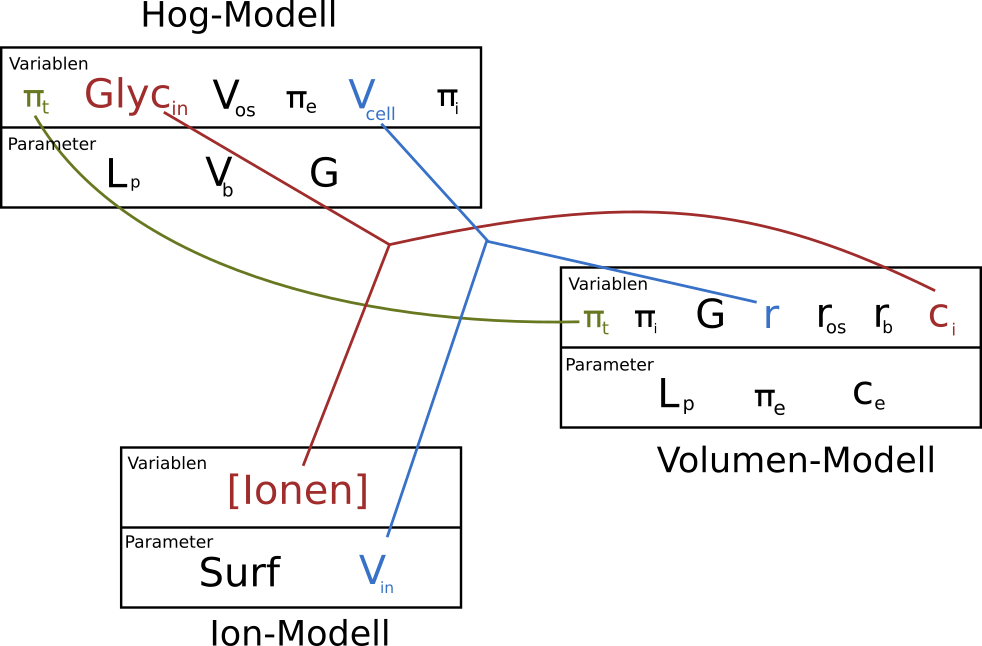
\includegraphics[width=\textwidth]{picture/model_intersections.png}
			\caption{intersections of the three models } 
			\label{IntersectionsOfTheModels} 
		\end{minipage}
	\end{center}
\end{figure}

In our momentan state of knowledge, there is not yet a model which integrate this three modules into a single model. The combined model simulates the interaction between extra- and intracellular ionconcentration, changes in cell volume and the activity of the MAP cascade (???). The model senses the differences in the osmolarity between the cell and its environment and adapt with the important Hog pathway with the MAP cascade the cell volume and the intracellular osmolyt concentrations. 

\subsection{theory}
The ion model consists out of a non-equivilibrium thermodynamic (NET) approach to model the transport of the ion over the plasma membrane. \\\\
In the ion model a glycerol stimulus is further simulated. \\
The cell volume depends essential on the relation of the internal, external and turgor pressure. The internal and external pressure $\pi$ depends on the concentration $c$ of the osmotic active substance in the corresponding areas correlated over the equation \ref{osmotic_pressure}
\begin{equation} \label{osmotic_pressure}
	\pi = c \cdot R \cdot T	
\end{equation} 




